\documentclass[12pt]{article}
\usepackage[margin=1in]{geometry}
\usepackage{graphicx}
\usepackage{amsmath}
\usepackage{hyperref}
\usepackage{appendix}
\usepackage{color}

\newcommand{\fixme}[1]{\textcolor{darkred}{\bf FIXME: #1}}
\newcommand{\s}[1]{{\mbox{\scriptsize #1}}}

\begin{document}

\section{Introduction}

The muon endcap was aligned using information from four different
sources: photogrammetry, the Muon Endcap Alignment System, tracks from
beam-halo muons, and tracks from collisions muons.  Some of these
sources of information are orthogonal, while others provide for
cross-checks between the different systems.  To combine information,
alignment corrections were applied in a well-defined sequence, such
that each step benefits from the previous.  Potentially interdependent
corrections were iterated to obtain a mutually consistent solution.

\begin{figure}
\begin{center}
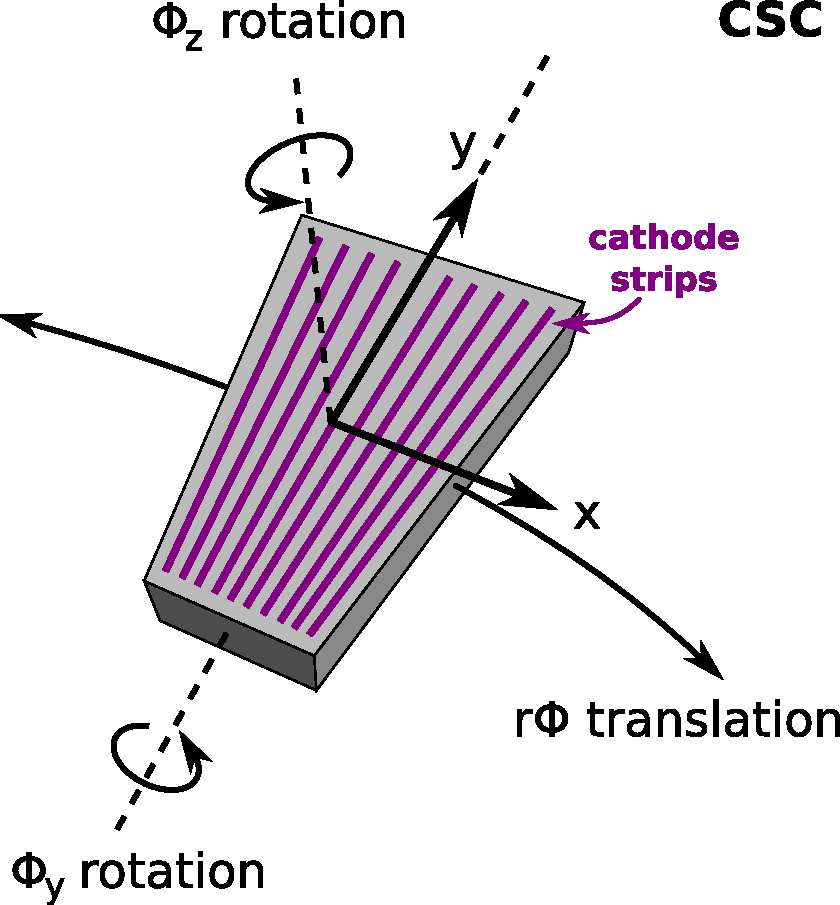
\includegraphics[width=0.3\linewidth]{csc_coordinates.pdf}

\caption{Schematic CSC chamber, indicating the local coordinate
  system. \label{fig:csc_coordinates}}
\end{center}

\end{figure}

\section{Measurement of disk bending with the Muon Endcap Alignment System}

\section{Internal-ring alignment using beam-halo tracks}

CSC chambers overlap slightly along their edges, and muons passing
through these narrow regions provide information about the relative
displacement of the neighboring chambers.  To produce a complete
geometry from the pairwise chamber information, the following
objective function is minimized:
\begin{equation}
\chi^2 = \sum_{m_{ij}}^\s{constraints} \frac{(m_{ij} - A_i +
  A_j)^2}{{\sigma_{ij}}^2} + \lambda \left(\frac{1}{N_\s{chambers}} \sum_i^\s{chambers}A_i\right)^2
\label{eqn:minimizeme}
\end{equation}
where $A_i$ are the chamber coordinates to optimize, $m_{ij} \pm
\sigma_{ij}$ are the pairwise chamber measurements, and $\lambda$ is a
Lagrange multiplier to constrain the floating coordinate system.  Two
types of constraints are used: beam-halo tracks and photogrammetry
measurements, with the latter applied only to pairs of chambers that
were missing track data due to inefficient read-out electronics (14
out of 396 pairs of neighboring chambers).  The alignment proceeds in
alternating passes, first aligning $r\phi$ positions ($A_i$ are
interpreted as positions and $m_{ij}$ are residuals), then $\phi_z$
angles ($A_i$ are chamber angles and $m_{ij}$ are
residuals-times-lever arm).  The alignment fully converged after one
$r\phi$ pass and one $\phi_z$ pass.

Although photogrammetry information was used to constrain a fraction
of the chambers, much larger weights were given to the beam-halo data,
in inverse proportion to the square of the measurement uncertainties
in the two methods.  As seen in Fig.~\ref{fig:aligned_minus_pg}, the
level of agreement between the track-based technique and
photogrammetry is 0.3--0.6~mm.  This is much smaller than the typical
scale of chamber corrections from design geometry (2--3~mm).

\begin{figure}
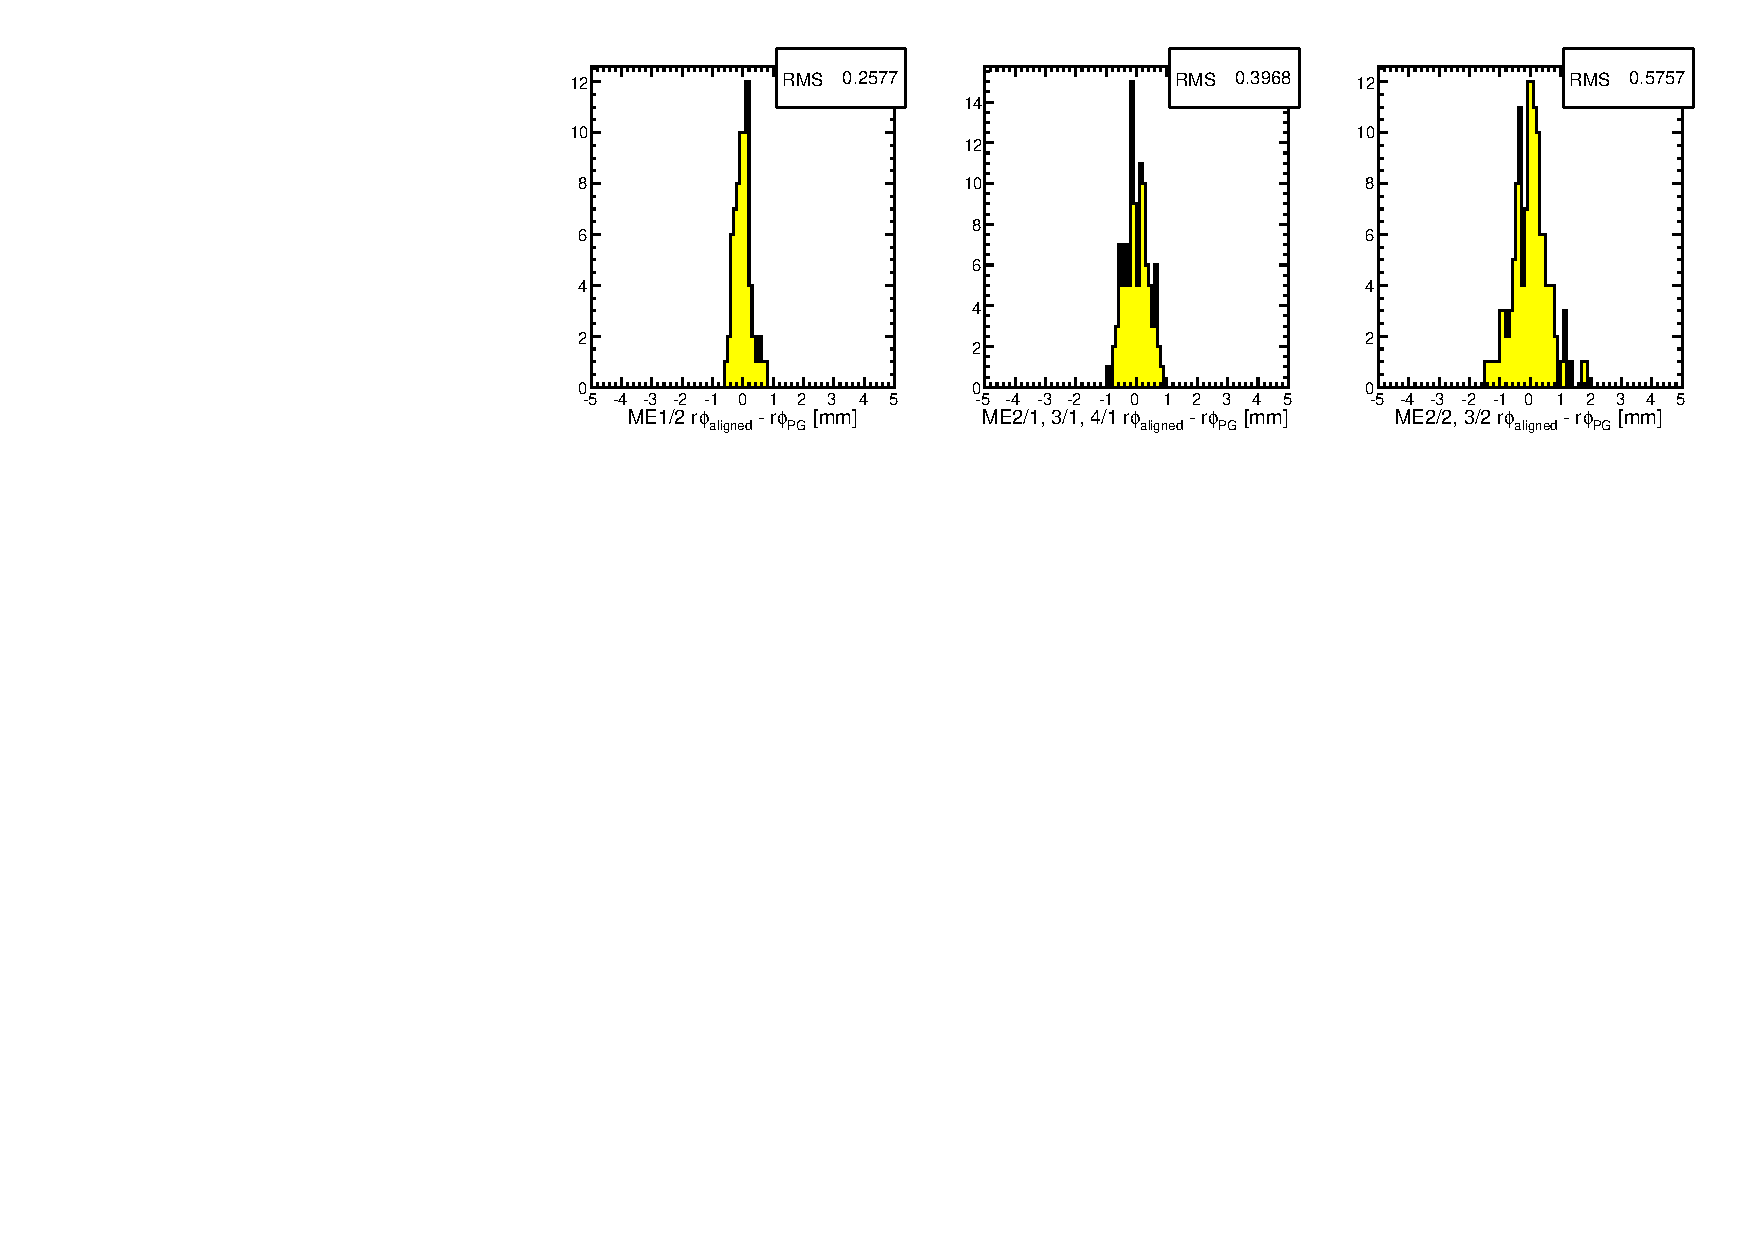
\includegraphics[width=\linewidth]{aligned_minus_pg.pdf}

\caption{Chamber positions after internal-ring alignment compared
  with photogrammetry, split by ring.  (ME1/1 chambers were not
  measured by the photogrammetry.) \label{fig:aligned_minus_pg}}
\end{figure}

\section{Whole-ring placement using collisions muons}

To complete the endcap alignment, the internally aligned rings must be
aligned relative to one another and the tracker.  Tracks from the
tracker were propagated to the muon chambers and whole-ring
corrections were derived from the pattern of $r\phi$ residuals as a
function of global $\phi$.  A constant offset in the residuals is
interpreted as a rotation of the ring in $\phi_z$, while terms
proportional to $\cos\phi$ and $\sin\phi$ are interpreted as
displacements in global $x$ and $y$, respectively.

Figure~\ref{fig:one_and_only_mapplot} provides an example of an
alignment fit for one ring (ME$-$2/1).  The alignment was performed in
one pass, with a second to verify self-consistency.

\begin{figure}
\begin{center}
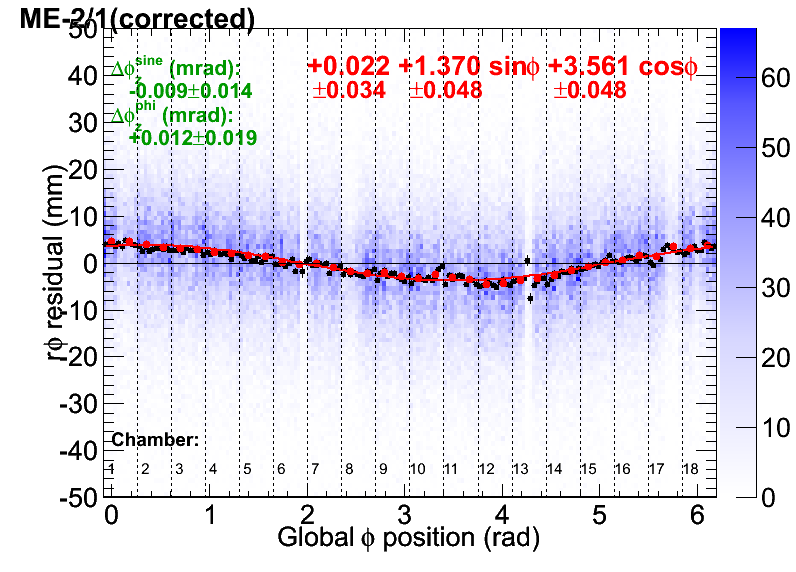
\includegraphics[width=0.5\linewidth]{one_and_only_mapplot.png}
\end{center}

\caption{Residuals plot used to align a ring: the color scale is the
  residuals distribution versus $\phi$, black points are a profile
  derived from truncated-Gaussian peak fits in each $\phi$ bin, and
  red points are the average of peak-fits to muons and antimuons
  separately.  The fitted curve is interpreted as three alignment
  degrees of freedom.  Vertical dashed lines indicate the boundaries
  between chambers. \label{fig:one_and_only_mapplot}}
\end{figure}

To cross-check the alignment using a qualitatively different method,
beam-halo tracks crossing an entire endcap (three or four stations,
depending on distance from the beamline) were used to calculate
residuals in one station relative to segments in another.
Figure~\ref{fig:BHCrossCheck_mep41} shows an example, in which
ME$+$3/1 segments were propagated linearly (no corrections for
material or magnetic field) to ME$+$4/1.  These plots were not used to
perform the alignment, so the fact that the strong $\phi$ trend
observed before alignment is eliminated in the aligned geometry adds
confidence to the result.

\begin{figure}
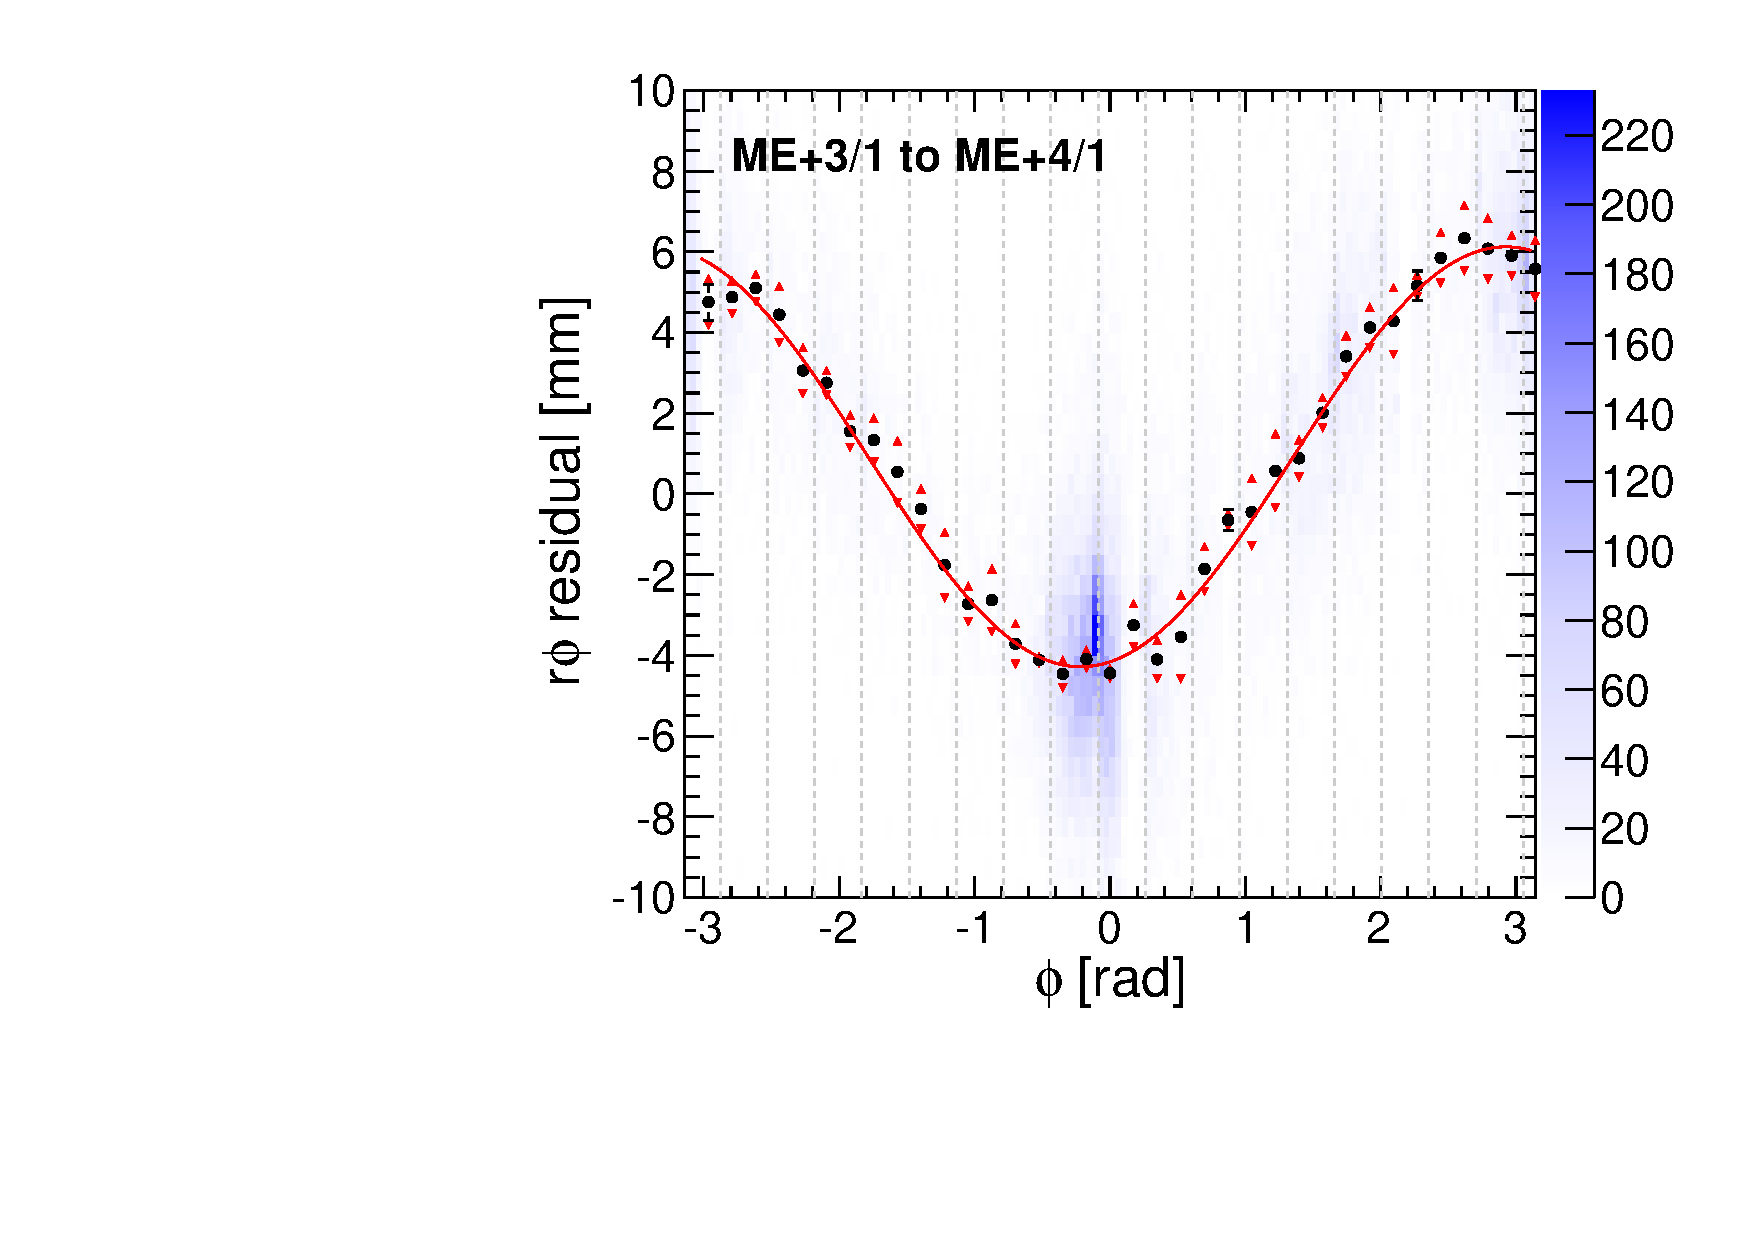
\includegraphics[width=0.45\linewidth]{BHCrossCheck_mep41_before.pdf} \hfill
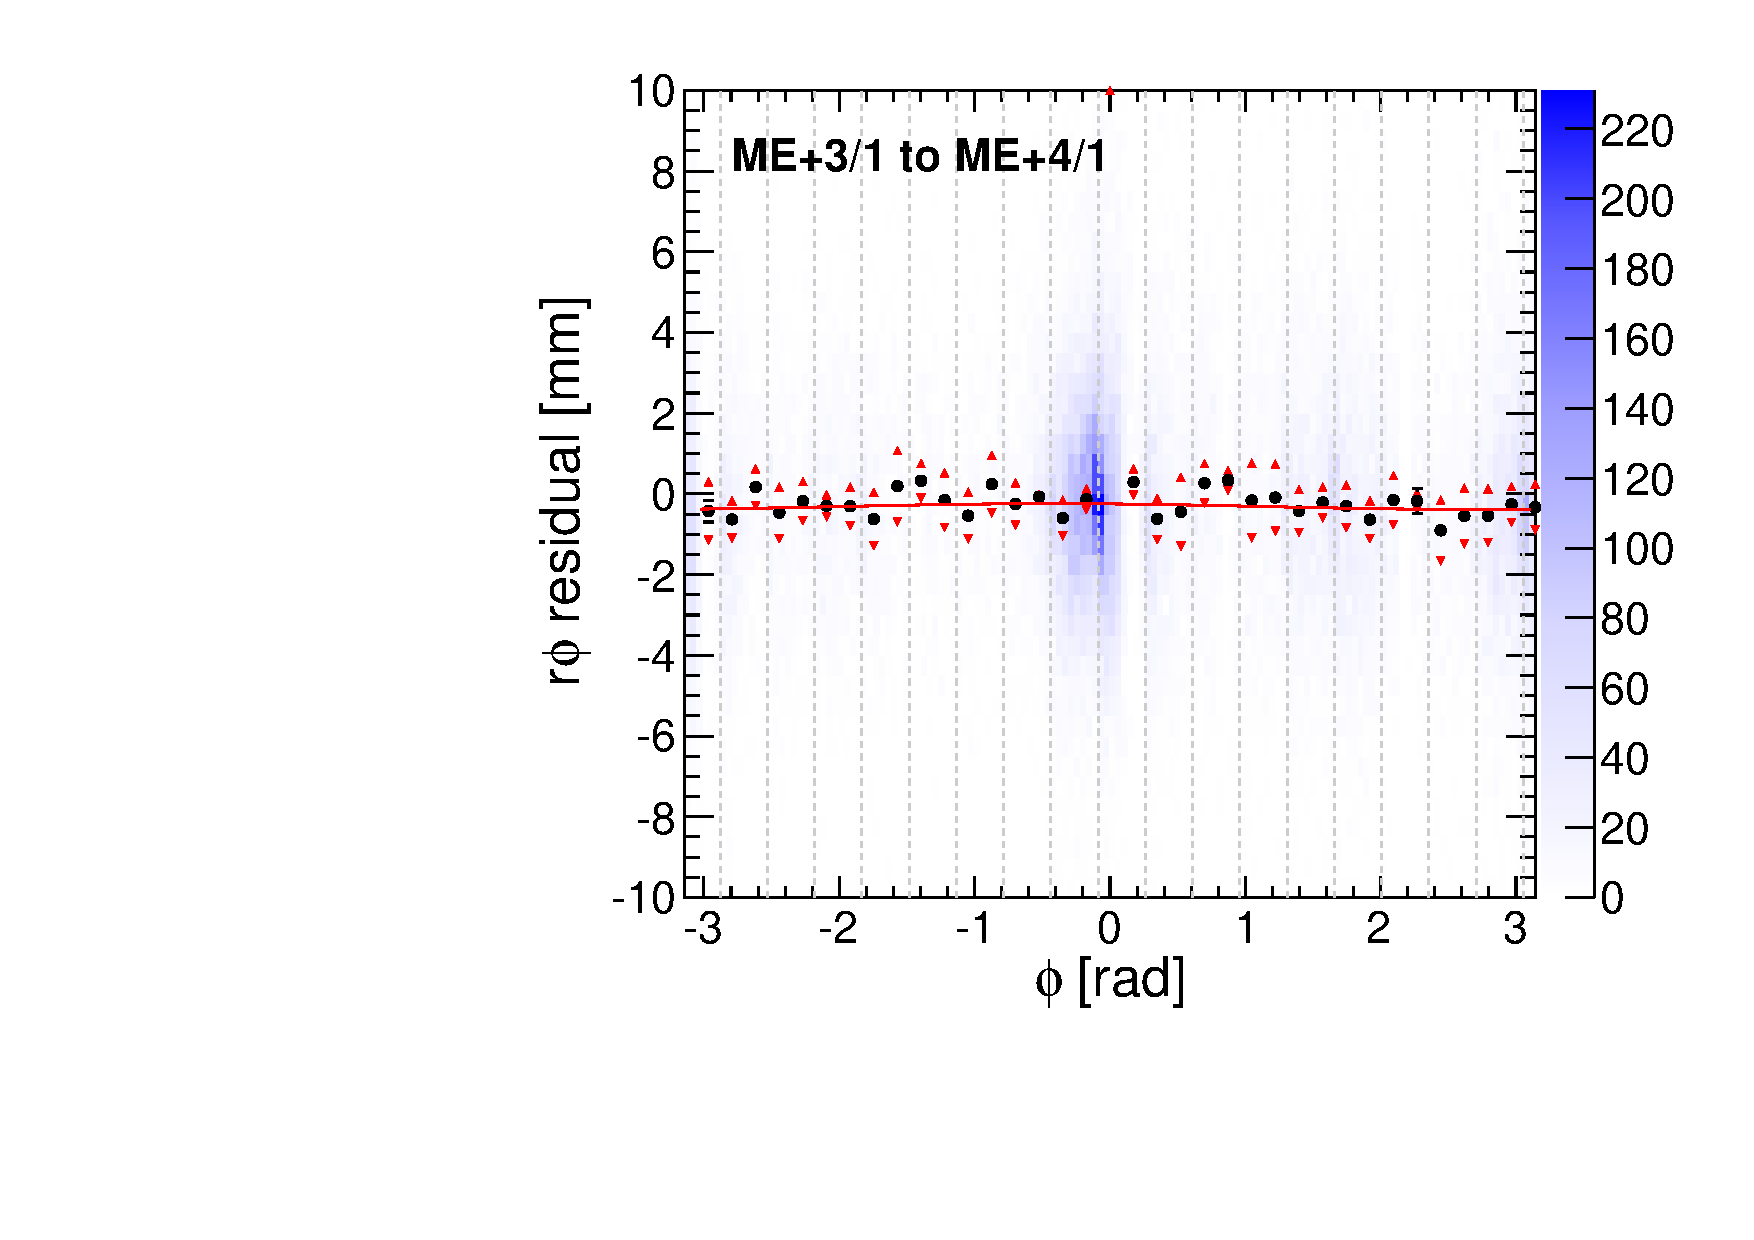
\includegraphics[width=0.45\linewidth]{BHCrossCheck_mep41_after.pdf}

\caption{Residuals from beam-halo tracks used to cross-check the
  alignment performed with collisions.  The symbols in these plots
  have the same meaning as Fig.~\ref{fig:one_and_only_mapplot}, though
  residuals were calculated differently (see text).  Left: before
  alignment.  Right: after alignment using collisions (not
  beam-halo).  \label{fig:BHCrossCheck_mep41}}
\end{figure}

\end{document}
